\documentclass[../main.tex]{subfiles}

\begin{document} %%%%%%%%%%%%%%%%%%%%%%%%%%%%%%%%%%%%%%%%%%%%%%%%%%%%%%%%%%%%
\section{Definiciones}
    \subsection{Varianza}
        \begin{definition}(Varianza).
            Sea $X$ una variable aleatoria con esperanza finita. La varianza de $X$ se define por
            \begin{equation}
                 Var(X) = E[(X - E[X])^2]
            \end{equation}
        \end{definition}

        \begin{definition}(Desviación estándar).
            La desviación estándar de $X$ se define por
            \begin{equation}
                \sigma_X = \sqrt{Var(X)}
            \end{equation}
        \end{definition}


    \subsection{Covarianza}
        \begin{definition}\textbf{(Covarianza)}
            La covarianza es una medida de cómo varían conjuntamente dos variables aleatorias.

            Sean $X$ e $Y$ dos variables aleatorias de varianzas finitas definidas sobre el mismo espacio de probabilidad $(\Omega ,A, P)$. La covarianza de $X$ e $Y$ se define por
            \begin{equation}
                \begin{split}
                    Cov(X,Y) &= E[(X - E[X])(Y - E[Y])] 
                    \\&= E[XY] - E[X]E[Y]
                \end{split}
            \end{equation}

            \underline{Interpretación de la covarianza:}
            \begin{itemize}
                \item Si $S_{xy} > 0$ hay dependencia directa (positiva), es decir, a grandes valores de $X$ corresponden grandes valores de $Y$.
                \item Si $S_{xy} < 0$ hay dependencia inversa (negativa), es decir, a grandes valores de $X$ corresponden pequeños valores de $Y$.
                \item Si $S_{xy} = 0$ no hay dependencia lineal entre $X$ e $Y$.
            \end{itemize}
    
            % cargamos imagen
            \begin{figure}[htb]
                \centering
                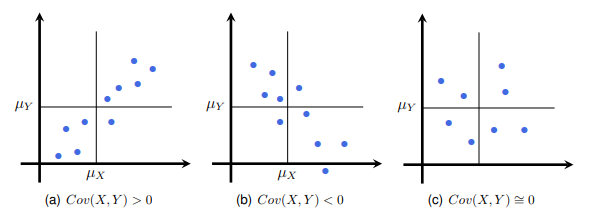
\includegraphics[scale=0.5]{./images/covarianza.png}
                \caption{Covarianza}
                \label{fig:covarianza}
            \end{figure}
            
        \end{definition}

        \begin{definition} (Covarianza muestral) 
            \begin{equation}
                S_{xy} = \frac{1}{n-1} \cdot \sum_{i=1}^{n}(x_i - \bar{x})(y_i - \bar{y})
            \end{equation}
        \end{definition}
        
        \begin{equation}
            \bar{x} = \frac{1}{n} \cdot \sum_{i=1}^{n} x_i \quad  \quad \quad \bar{y} = \frac{1}{n} \cdot \sum_{i=1}^{n} y_i
        \end{equation}

        \begin{definition} (Coeficiente de Correlación de Pearson)
            \begin{equation}
                \begin{split}
                    \rho_{xy} &= \frac{S_{xy}}{S_x \cdot S_y}
                    \\&= \frac{\sum_{i=1}^{n} (x_i - \bar{x}) \cdot (y_i - \bar{y})}{\sum_{i=1}^{n} (x_i - \bar{x})^2 \cdot \sum_{i=1}^{n} (y_i - \bar{y})^2}
                \end{split}
            \end{equation}

            % cargamos imagen
            \begin{figure}[htb]
                \centering
                \includegraphics[scale=0.4]{./images/coeficiente_correlación.png}
                \caption{Coeficiente de Correlación de Pearson}
                \label{fig:coeficiente_correlación}
            \end{figure}
        \end{definition}



\end{document}  %%%%%%%%%%%%%%%%%%%%%%%%%%%%%%%%%%%%%%%%%%%%%%%%%%%%%%%%%%%%%